%%%%%%%%%%%%%%%%%%%%%%%%%%%%%%%%%%%%%%%%
% Beamer Presentation
% LaTeX Template
% Version 1.0 (10/11/12)
%
% This template has been downloaded from:
% http://www.LaTeXTemplates.com
%
% License:
% CC BY-NC-SA 3.0 (http://creativecommons.org/licenses/by-nc-sa/3.0/)
%
%%%%%%%%%%%%%%%%%%%%%%%%%%%%%%%%%%%%%%%%%

%----------------------------------------------------------------------------------------
%	PACKAGES AND THEMES
%----------------------------------------------------------------------------------------

\documentclass[xcolor=dvipsnames, aspectratio=169]{beamer}

\mode<presentation> {

% The Beamer class comes with a number of default slide themes
% which change the colors and layouts of slides. Below this is a list
% of all the themes, uncomment each in turn to see what they look like.

\usetheme{Madrid} %Hannover
% As well as themes, the Beamer class has a number of color themes
% for any slide theme. Uncomment each of these in turn to see how it
% changes the colors of your current slide theme.
\useoutertheme{infolines} % Alternatively: miniframes, infolines, split
\useinnertheme{circles}
\definecolor{UBCblue}{rgb}{0.04706, 0.13725, 0.26667} % UBC Blue (primary)
\usecolortheme[named=UBCblue]{structure}
}

\usepackage{graphicx} % Allows including images
\usepackage{booktabs} % Allows the use of \toprule, \midrule and \bottomrule in tables
\usepackage{textpos}
\usepackage{caption}
\usepackage[utf8]{inputenc}
\usepackage[brazilian]{babel}
\usepackage{csquotes}
\usepackage{listings}
\setbeamertemplate{caption}[numbered]
\usepackage[style=abnt]{biblatex}
\addbibresource{bibliography.bib}
\PassOptionsToPackage{useregional}{datetime2}
\usepackage{xcolor}


\definecolor{codegreen}{rgb}{0,0.6,0}
\definecolor{codegray}{rgb}{0.5,0.5,0.5}
\definecolor{codepurple}{rgb}{0.58,0,0.82}
\definecolor{backcolour}{rgb}{0.95,0.95,0.92}
\definecolor{string-color}{rgb}{0.3333, 0.5254, 0.345}

\lstdefinestyle{mystyle}{
    backgroundcolor=\color{backcolour},   
    commentstyle=\color{codegreen},
    keywordstyle=\color{string-color},
    keywordstyle=[2]{\color{codepurple}},
    keywordstyle=[3]{\color{magenta}},
    numberstyle=\tiny\color{codegray},
    stringstyle=\color{codepurple},
    basicstyle=\ttfamily\footnotesize,
    breakatwhitespace=false,         
    breaklines=true,                 
    captionpos=b,                    
    keepspaces=true,                 
    numbers=left,                    
    numbersep=5pt,                  
    showspaces=false,                
    showstringspaces=false,
    showtabs=false,                  
    tabsize=2,
    otherkeywords = {tf, Sequential, SimpleRNN, Dense, GRU, LSTM},
    morekeywords = [3]{keras},
}

\lstset{style=mystyle}
\newcommand{\source}[1]{\vspace{-20pt} \caption*{ Fonte: {#1}} }
\usepackage{copyrightbox}


\makeatletter
% \beamer@nav@subsectionstyle{hide/hide/hide}
\addtobeamertemplate{sidebar left}{%
\hspace{0.5cm}
\includegraphics[width=0.9cm, keepaspectratio]{figures/_brasao_ufsm_cor.png}
% \hspace{2.3cm}
\includegraphics[width=0.8cm, keepaspectratio]{figures/brasao_ctism.png}
% \hspace{2.3cm}\includegraphics[width=1.5cm, keepaspectratio]{_logosbc.png}
% \hspace{2.3cm}\includegraphics[width=1.5cm, keepaspectratio]{_logoERRC.png}%
}{}


\setbeamertemplate{footline}
{
	\leavevmode%
	\hbox{%
	    %\hspace{0.25cm}
\includegraphics[width=2cm, keepaspectratio]{figures/brasao_ufsm_cor.png}
		\begin{beamercolorbox}[wd=.333333\paperwidth,ht=2.25ex,dp=1ex,right]{date in head/foot}%
			\usebeamerfont{date in head/foot}\insertshortdate{}\hspace*{2em}
			\insertframenumber{} / \inserttotalframenumber\hspace*{2ex} 
		\end{beamercolorbox}}%
		%\vskip0pt%
	}
\makeatother

%----------------------------------------------------------------------------------------
%	TITLE PAGE
%----------------------------------------------------------------------------------------

\title[]{Frequency Modulation} % The short title appears at the bottom of every slide, the full title is only on the title page

\author[]{Fábio Demo da Rosa} % Your name
%\includegraphics[]{logositeredes.png}
\institute[UFSM] % Your institution as it will appear on the bottom of every slide, may be shorthand to save space
{
Universidade Federal de Santa Maria \\ % Your institution for the title page
Pós-Graduação em Ciência da Computação \\
Disciplina de Robótica Móvel\\
\medskip
\textit{faberdemo@gmail.com} % Your email address
}
\date{25 de Agosto de 2023} % Date, can be changed to a custom date
\newcounter{saveenumi}
\newcommand{\seti}{\setcounter{saveenumi}{\value{enumi}}}
\newcommand{\conti}{\setcounter{enumi}{\value{saveenumi}}}

\resetcounteronoverlays{saveenumi}


\begin{document}

\begin{frame}
\titlepage % Print the title page as the first slide
\end{frame}

\begin{frame}
\frametitle{Visão Geral} %\includegraphics[]{logositeredes.png}} % Table of contents slide, comment this block out to remove it
\tableofcontents % Throughout your presentation, if you choose to use \section{} and \subsection{} commands, these will automatically be printed on this slide as an overview of your presentation
\end{frame}

%----------------------------------------------------------------------------------------
%	PRESENTATION SLIDES
%----------------------------------------------------------------------------------------

%------------------------------------------------
\section[Introdução]{Frequency Modulation} 
%------------------------------------------------
\begin{frame}[allowframebreaks, fragile]
\frametitle{Frequency Modulation}
	\begin{itemize}
		\item O \textit{Frequency Modulated Continuous Wave Radar} (FMCW), ou Radar de Onda contínua com Modulação de Frequência, é uma técnica alternativa ao Phase-shift measurement;
		\item Transmissão de uma onda eletromagnética contínua modulada por um sinal triangular periódico que ajusta a frequência da portadora acima e abaixo da frequência média f0;
		\item O transmissor emite um sinal que varia em frequência como uma função linear do tempo;
		\begin{equation}
            f(t) = f_0 + at
        \end{equation}
        \item Onde:
        \begin{itemize}
            \item[] $a$ = \textit{some constant};
            \item[] $t$ = \textit{elapsed time}.
        \end{itemize}
        \item O sinal é refletido no alvo e chega ao receptor em um tempo $t + T$
        \begin{equation}
            T = \frac{2d}{c}
        \end{equation}
        \item Onde:
        \begin{itemize}
            \item[] $T$ = \textit{round-trip propagation time};
            \item[] $d$ = \textit{distance to target};
            \item[] $c$ = \textit{speed of light}.
        \end{itemize}
        \begin{figure}
            \centering
            \copyrightbox[b]{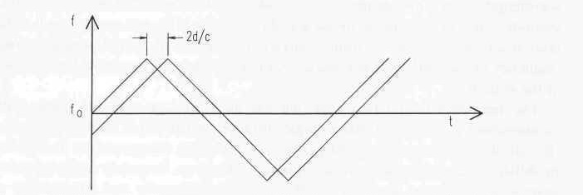
\includegraphics[scale=0.55]{figures/1_curva_de_frequencia.png}}%
            {Fonte: \cite{everett1995sensors}}
            \caption{A curva de frequência recebida é deslocada ao longo do eixo do tempo em relação à frequência de referência.}
            \label{fig:curva_de_freq}
        \end{figure}
        \item O sinal recebido é comparado com o sinal referência obtido diretamente do transmissor;
        \item A curva de frequência recebida será deslocada ao longo do eixo de tempo, por um período igual ao tempo necessário para a onda se propagar e retornar;
        \item Devido ao efeito Doppler, pode ocorrer um deslocamento no eixo de frequência.
        \item As duas frequências da \ref{fig:curva_de_freq}, quando combinadas em um misturador, produzem uma frequência de batida $f_{b}$:
        \begin{equation}
            F_{b} = f(t) - f(T + t) = aT
        \end{equation}
        \item A \textit{frequency beat} é a medida usada para calcular a distância do objeto (alvo):
        \begin{equation}
            d = \frac{F_{b}c}{4F_{r}F{_d}}
        \end{equation}
        \item Onde:
        \begin{itemize}
            \item[] $c$ = range to target;
            \item[] $d$ = speed of light;
            \item[] $F_{b}$ = \textit{beat frequency};
            \item[] $F_{r}$ = \textit{repetition (modulation) frequency};
            \item[] $F_{d}$ = \textit{total FM frequency deviation}.
        \end{itemize}
        \item A medida da distância é proporcional a diferença ou \textit{frequency beat};
        \item Os avanços no controle de onda de diodos laser permite essa tecnologia de alcance com radar ser usada com lasers.
        \item A \textit{frequency-modulation} apresenta vantagens sobre a \textit{phase-shift measurement}, já que não apresenta ambiguidade quando medindo uma única distância;
        \item Entretanto, possui desvantagens associadas com a linearidade e repetibilidade da \textit{frequency ramp}, assim como a coerência do feixe de laser em sistemas ópticos;
        \item Sendo assim, a maioria dos FMCW disponíveis comercialmente são baseados em radar, enquanto os dispositivos laser são mais comuns no TOF ou no \textit{phase-detection}
	\end{itemize}
\end{frame}


%------------------------------------------------
\section[VRSS Automotive Collision Avoidance Radar]{VRSS Automotive Collision Avoidance Radar} 
%------------------------------------------------

\begin{frame}[allowframebreaks, fragile]
\frametitle{Automotive Collision Avoidance Radar}
	\begin{itemize}
		\item É um radar Doppler modificado, com intuito de alertar motoristas para situações perigosas;
		\item uma antena de microondas miniaturizada, montada no parachoque do veículo envia um sinal de feixe estreito que detecta apenas os objetos diretamente no caminho do veículo
        \begin{itemize}
            \item ignorando alvos (placas de trânsito e carros estacionados) em ambas as vias.
        \end{itemize}
        \item Quando o sinal do radar é refletido por um alvo estacionário ou em movimento mais lento, ele é detectado pela antena e transmitido a um processador de sinal eletrônico sob o capô.
        \item O processador de sinal computa constantemente:
        \begin{itemize}
            \item Velocidade deo veículo;
            \item Aceleração;
            \item Distância do alvo;
            \item Velocidade relativa.
        \end{itemize}
        \item Se algum desses parâmetros necessitem que o motorista tome uma ação ofensiva/corretiva, um \textit{buzzer} e uma luz são ativadas em um painel "especial" do veículo.
        \begin{figure}
            \centering
            \copyrightbox[b]{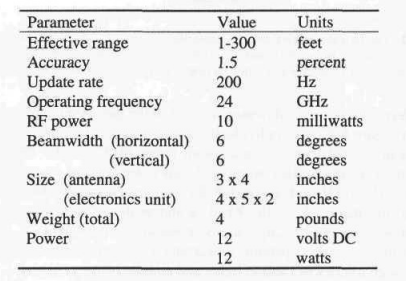
\includegraphics[scale=0.4]{figures/2_VRSS_specs.png}}%
            {Fonte: \cite{everett1995sensors}}
            \caption{Especificações VRSS}
            \label{fig:curva_de_freq}
        \end{figure}
	\end{itemize}
\end{frame}


%------------------------------------------------
\section[VORAD Vehicle Detection and Driver Alert System]{VORAD Vehicle Detection and Driver Alert System} 
%------------------------------------------------

\begin{frame}[allowframebreaks, fragile]
\frametitle{Vehicle Detection and Driver Alert System}
	\begin{itemize}
		\item VORAD (\textit{Vehicle Onboard Radar}) Safety Systems, Inc., também desenvolveu um sistema comercial de radar doppler FMCW de ondas milimétricas;
        \begin{figure}
            \centering
            \copyrightbox[b]{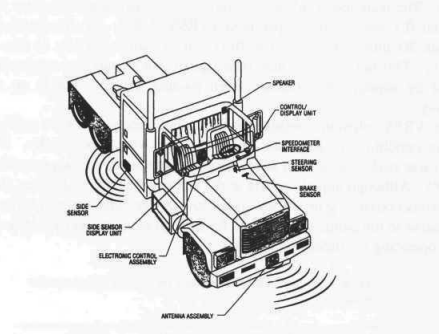
\includegraphics[scale=0.35]{figures/3_VORAD.png}}%
            {Fonte: \cite{everett1995sensors}}
            \caption{O módulo antena/trasmissor/receptor é montado na frente (ou lateral) do veículo}
            \label{fig:curva_de_freq}
        \end{figure}
		\item O VORAD consegue distinguir até 20 objetos estacionários ou em movimento, dentro de um \textit{range} de 350 pés (106,68m);
		\item Dois microprocessadores calculam o \textit{range} e a \textit{range-rate} dos dados (radio frequência) e analisam os resultados em conjunto com a velocidade, frenagem e ângulo da direção;
		\item Esse ssitema também guarda 20 minutos dos dados históricos mais recentes numa memória EEPROM para reconstrução dos fatos após possíveis acidentes.
	\end{itemize}
\end{frame}


%------------------------------------------------
\section[Safety First System Vehicular Obstacle Detection and Warning System]{Safety First System Vehicular Obstacle Detection and Warning System} 
%------------------------------------------------

\begin{frame}[allowframebreaks, fragile]
\frametitle{Safety First System Vehicular Obstacle Detection and Warning System}
	\begin{itemize}
		\item A
        \begin{figure}
            \centering
            \copyrightbox[b]{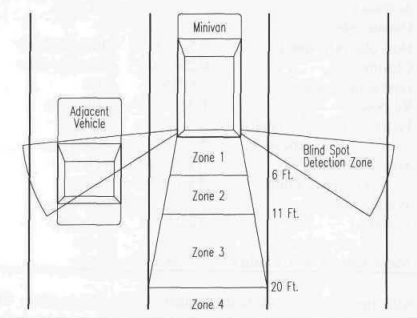
\includegraphics[scale=0.35]{figures/4_safety_first_system.png}}%
            {Fonte: \cite{everett1995sensors}}
            \caption{Safety First System}
            \label{fig:curva_de_freq}
        \end{figure}

        \item B

        \begin{figure}
            \centering
            \copyrightbox[b]{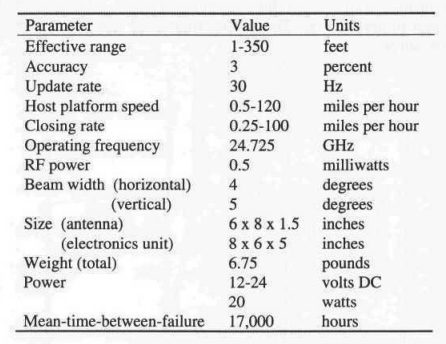
\includegraphics[scale=0.35]{figures/5_VORAD_specs.png}}%
            {Fonte: \cite{everett1995sensors}}
            \caption{O módulo antena/trasmissor/receptor é montado na frente (ou lateral) do veículo}
            \label{fig:curva_de_freq}
        \end{figure}
	\end{itemize}
\end{frame}


%------------------------------------------------
\section[Millitech Millimiter Wave Radar]{Millitech Millimiter Wave Radar} 
%------------------------------------------------

\begin{frame}[allowframebreaks, fragile]
\frametitle{Millitech Millimiter Wave Radar}
	\begin{itemize}
		\item Semelhante a uma Feedforward Neural Network, sem conexões apontando para trás;
        \begin{figure}
            \centering
            \copyrightbox[b]{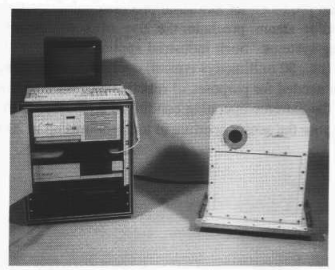
\includegraphics[scale=0.35]{figures/6_militech_wave_radar.png}}%
            {Fonte: \cite{everett1995sensors}}
            \caption{O módulo antena/trasmissor/receptor é montado na frente (ou lateral) do veículo}
            \label{fig:curva_de_freq}
        \end{figure}

        \item B
        
        \begin{figure}
            \centering
            \copyrightbox[b]{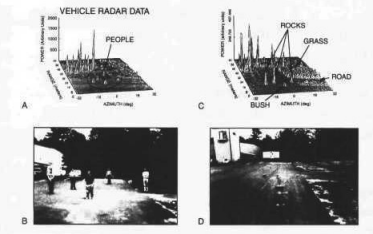
\includegraphics[scale=0.65]{figures/7_militech_wave_radar_range_scanned_data.png}}%
            {Fonte: \cite{everett1995sensors}}
            \caption{Dados obtidos (escaneados) com sensor de 256-pixels}
            \label{fig:militech_sensor_data}
        \end{figure}


        \item c

        \begin{figure}
            \centering
            \copyrightbox[b]{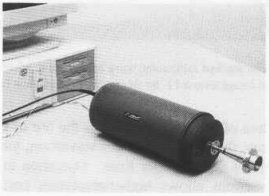
\includegraphics[scale=0.35]{figures/8_militech_wave_radar_industry_sensor.png}}%
            {Fonte: \cite{everett1995sensors}}
            \caption{Os sensores de onda milimétricas FMCW são protegidos contra altas temperaturas}
            \label{fig:militech_sensor_}
        \end{figure}
        
        \item d


        \begin{figure}
            \centering
            \copyrightbox[b]{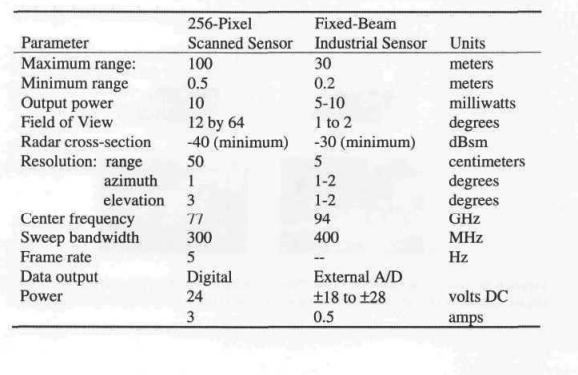
\includegraphics[scale=0.35]{figures/9_militech_wave_radar_specs.png}}%
            {Fonte: \cite{everett1995sensors}}
            \caption{Especificações do Millitech Millimiter Wave Radar}
            \label{fig:militech_specs}
        \end{figure}

	\end{itemize}
\end{frame}


%------------------------------------------------
%\section*{Referências}
%------------------------------------------------

\begin{frame}
    % \nocite{*}
    \printbibliography
\end{frame}


\begin{frame}
\titlepage % Print the title page as the first slide
\end{frame}

\end{document}